\documentclass[useAMS,usenatbib]{mn2e}

\voffset=-0.8in

% Packages:
\usepackage{graphicx}
\usepackage{amsmath}
\usepackage{xspace}
\usepackage{dsfont}

% Bold symbols
\renewcommand{\btheta}{\boldsymbol{\theta}}
\newcommand{\bdata}{\boldsymbol{D}}
\newcommand{\bx}{\{x_i\}}

% \onecolumn
%%%%%%%%%%%%%%%%%%%%%%%%%%%%%%%%%%%%%%%%%%%%%%%%%%%%%%%%%%%%%%%%%%%%%%%%%%%%%%

\title[]
{Fast Bayesian Inference for Exoplanet Discovery in Radial Velocity Data}
    
\author[Brewer and Donovan]{%
  Brendon~J.~Brewer$^{1}$\thanks{bj.brewer@auckland.ac.nz},
  Courtney P. Donovan$^{1}$
  \medskip\\
  $^1$Department of Statistics, The University of Auckland, Private Bag 92019, Auckland 1142, New Zealand}

%%%%%%%%%%%%%%%%%%%%%%%%%%%%%%%%%%%%%%%%%%%%%%%%%%%%%%%%%%%%%%%%%%%%%%%%%%%%%%

\begin{document}
             
\date{To be submitted to MNRAS}
             
\maketitle

\label{firstpage}

%%%%%%%%%%%%%%%%%%%%%%%%%%%%%%%%%%%%%%%%%%%%%%%%%%%%%%%%%%%%%%%%%%%%%%%%%%%%%%

\begin{abstract}
Inferring the number of planets $N$ in an exoplanetary system from radial velocity
(RV) data is a challenging task. Recently, it has become clear that RV data
can contain periodic signals due to stellar activity, which can be difficult
to distinguish from planetary signals. However, even doing the inference
under a given set of siplifying assumptions (e.g. no stellar activity) can
be difficult. It is common for the posterior distribution for the
planet parameters, such as orbital periods,
to be multimodal and to have other awkward features. In
addition, when $N$ is unknown, the marginal likelihood (or evidence), as a
function of $N$, is required. Rather than doing separate runs with different
values of $N$, we propose an alternative
approach using a trans-dimensional Markov Chain Monte Carlo method within
Nested Sampling. The posterior distribution for $N$ can be obtained with a
single run, which takes $\sim$ 15 minutes on a typical modern desktop computer.
We apply the method to $\nu$ Oph and Gliese 581, finding moderate evidence
(posterior probability of existence = 70\%) for a third signal in
$\nu$ Oph with an orbital period of 75.7 $\pm$ 1.8 days. The results also
suggest Gliese 581 hosts many (7-15) ``planets'' (or other causes of other periodic
signals), but only four have well determined periods. The analysis of both
of these datasets shows phase transitions exist which are difficult to
negotiate without Nested Sampling.
\end{abstract}

\begin{keywords}
stars: planetary systems --- techniques: radial velocities ---
methods: data analysis --- methods: statistical
\end{keywords}

%%%%%%%%%%%%%%%%%%%%%%%%%%%%%%%%%%%%%%%%%%%%%%%%%%%%%%%%%%%%%%%%%%%%%%%%%%%%%%

\section{Introduction}
The number of known extrasolar planets has exploded in the last two
decades, driven by improvements in
all of the different techniques used to detect and characterise exoplanets,
including the radial velocity (RV) method \citep[e.g.][]{2012PASJ...64..135S},
the transit method \citep[e.g.]{2014PNAS..11112647B},
and gravitational microlensing
\citep[e.g.][]{2014ApJ...785..155B, 2014ApJ...790...14Y}.

The problem of inferring the properties of an
exoplanetary system from observational data can be challenging.
In the particular case of radial velocity data,
the expected signal due to an exoplanet is periodic, and the goal is to
infer the number of planets in the system, as well as their properties such
as orbital periods and eccentricities. Many
different techniques have been proposed for doing this.
These techniques fall into two main
classes: i) those based on periodograms \citep[e.g.][]{2009A&A...496..577Z},
and ii) those based on model fitting in the Bayesian inference framework,
to describe the uncertainties probabilistically
\citep[e.g.][]{2011MNRAS.410...94G, 2014MNRAS.437.3540F,
2011A&A...528L...5T, fengji}. Bayesian model fitting via Markov Chain Monte
Carlo (MCMC) tends to be very computationally intensive, especially if we
want to calculate the posterior distribution for $N$, the number of planets.

It is now well known that RV datasets can contain periodic signals
resulting from stellar activity rather than planets \citep{2014Sci...345..440R}.
Therefore, it is important to develop models which attempt to distinguish
stellar activity signals from Keplerian planet signals based on the shape of
the oscillations and/or additional data constraining the periods of any
stellar activity signals. We do not address this important challenge in the
present paper. Rather, we consider the problem of inferring the number $N$ of
Keplerian signals in an RV dataset in a computationally efficient way.

We introduce a trans-dimensional birth-death MCMC approach
\citep{birthdeath} to inferring $N$.
When $N$ is treated as just another model parameter, we can obtain its
posterior distribution in a single run.
The exploration is done using Diffusive Nested Sampling
\citep[DNS][]{dnest} which replaces the posterior distribution with an alternative
{\it mixture of constrained priors}, allowing mixing between separated modes.
As a result, we are able to sample the posterior distribution for $N$, and
evaluate the marginal likelihood (including the sum over $N$) in
a single run which takes about 10 minutes on a 2-3 planet system.
On the other hand the approach of
\citet{2011MNRAS.410...94G} takes approximately 30 minutes per planet
(Gregory, priv. comm.). A C++ implementation of our method is available online
at {\tt https://github.com/eggplantbren/Exoplanet} under the terms of the
GNU General Public Licence version 3.

Computing the expected RV signal from
a planet in an elliptical orbit can be slow. Therefore we use a lookup table
of precomputed orbits, allowing us to do $\sim 15000$ MCMC steps per second
per CPU core.

\section{Inference}
Bayesian inference is the use of probability theory to describe uncertainty
\citep{sivia, ohagan}. In this framework, we approach data analysis problems by first
constructing a {\it hypothesis space}, which is the set of possible answers
to the problem we are considering. Normally, this is the set of possible
values of a vector of parameters $\btheta$ whose values we want
to know. We then assign probability distributions
called the {\it prior} and the {\it sampling distribution}. The prior
distribution $p(\btheta)$ describes
our initial uncertainty about which values of the parameters
$\btheta$ are plausible, and the
sampling distribution $p(\bdata | \btheta)$ describes
our initial uncertainty about the data set we're going to observe, as a
function of the unknown parameters $\btheta$.
When the data is known, our state of knowledge about the parameter is
updated from the prior $p(\theta)$ to the posterior distribution given by
Bayes' rule:
\begin{eqnarray}
p(\btheta | \bdata) &=&
\frac{p(\btheta)p(\bdata | \btheta)}
{p(\bdata)}
\end{eqnarray}
where $p(\bdata | \btheta)$ is called the likelihood, once the actual dataset
is substituted in.
The denominator, often called the {\it evidence} or
{\it marginal likelihood}, is given by the expected value of the likelihood
with respect to the prior:
\begin{eqnarray}
\mathcal{Z} = p(\bdata) = \int p(\btheta) p(\bdata | \btheta) d^n \btheta
\end{eqnarray}
where the integral is over the entire $n$-dimensional parameter space.

\subsection{Inferring the number of planets}
The number of orbiting planets, $N$, is an important parameter.
To calculate the posterior distribution for $N$, most authors
consider various trial values of $N$, and calculate the marginal likelihood
\begin{eqnarray}
p(\bdata | N) &=& \int p(\btheta | N) p(\bdata | \btheta, N) \, d^n \btheta
\end{eqnarray}
for each possible value of $N$
\citep[e.g.][]{2011MNRAS.415.2523G, 2011MNRAS.415.3462F, 2014MNRAS.437.3540F, fengji}, marginalising
over all other model parameters.
The posterior distribution for $N$ can then be found straightforwardly by
using Bayes' rule with $N$ as the only unknown parameter:
\begin{eqnarray}
p(N | \bdata) &=& \frac{p(N)p(\bdata | N)}{\sum_N p(N)p(\bdata | N)}.
\end{eqnarray}
Popular
methods for calculating the marginal likelihood are Nested Sampling
\citep{skilling} and ideas related to thermodynamic integration
\citep[e.g.][]{neal}. Note that thermodynamic integration can easily fail if
there is a phase transition in the problem \citep{skilling}.

This traditional approach can be very time consuming.
Methods for calculating the marginal likelihood are
already more intensive than standard MCMC methods for sampling the posterior,
because they usually involve a sequence of probability distributions
(e.g. the constrained priors in Nested Sampling, or the annealed distributions
in thermodynamic integration) rather than a single distribution (the posterior).
This intensive process needs to be run many times, for $N=0$, $N=1$, $N=2$, and
so on.

The traditional approach to inferring $N$ also contradicts
fundamental ideas in Bayesian
computation. Imagine we are trying to compute the posterior distribution for
a parameter $a$ in the presence of a nuisance parameter $b$. This is usually solved
by exploring the joint posterior for $a$ and $b$, and then only looking at the
generated values of $a$. Nobody would suggest the wasteful alternative
of using a discrete grid of possible $a$ values and doing an entire Nested
Sampling run for each, to get the marginal likelihood as a function of $a$.
Yet when the hypothesis space for $a$ is discrete to begin with, the wasteful
alternative has somehow become standard practice.

\subsection{Trans-dimensional MCMC}
Trans-dimensional MCMC methods such as birth-death MCMC \citep{birthdeath} or the
more general reversible jump MCMC \citep{green} treat the model dimension
$N$ as just another model parameter. At fixed $N$, standard techniques such
as the Metropolis algorithm can be used to explore the posterior distribution.
Additional moves that propose to change the value of $N$ are also defined. The
simplest of these are birth-death moves. More complicated moves, such as
split-and-merge \citep[e.g.][]{umstatter} are possible but usually not necessary.

In the exoplanet context, a birth move
proposes to add one more planet to the model. The new planet's properties
(period, amplitude, eccentricity, etc) are drawn from their prior distribution
which may depend on other other model parameters or hyperparameters.
The corresponding death move simply chooses a planet currently in the model,
and removes it. The acceptance probability for these moves is 1 if we want
to explore the prior. To implement these moves in Nested Sampling
\citep{skilling}, where the target distribution is proportional to the prior but with a hard likelihood
constraint, then the acceptance probability is 1 if the proposed move
satisfies the likelihood constraint, and 0 if it does not.

A recent paper \citep{rjobject} introduced a general approach to implementing
trans-dimensional models within Diffusive Nested Sampling \citep{dnest}, a
general MCMC algorithm. The \citet{rjobject} software predefines the
Metropolis proposals for exploring trans-dimensional target distributions,
including when the prior for the properties of each model component (i.e. each
planet) is defined hierarchically.

To fit a planet model to RV data, we need parameters to describe
the properties of each planet. For simplicity, we describe each planet by
five parameters: $T_i$, the orbital period, $A_i$, the amplitude (in metres
per second) of the RV signal, $\phi_i$, the phase of the signal, $v_i$, an
``initial velocity'' parameter describing the eccentricity of the orbit
(see Section~\ref{sec:orbits}), and $\theta_i$, a ``viewing angle'' parameter
describing the position of the observer with respect to the major axis of the
star's elliptical trajectory.

We assigned hierarchical priors to some of the planet's parameters. This allows the
model to capture the idea that knowing the values of some planet's parameters
provides some information about the parameters of another planet. Not using
hierarchical priors usually implies a strong prior commitment to the hypothesis
that the properties of the planets are spread out across the whole domain of
possible values, which is not necessarily the case.

The unknown parameters are:
\begin{eqnarray}
\left\{N, \boldsymbol{\alpha}, \{\boldsymbol{\psi}\}_{i=1}^N, y_0, s, \nu\right\}
\end{eqnarray}
where $N$ is the number of planets,
$\boldsymbol{\alpha} = \{\mu_T, \sigma_T, \mu_A\}$ are the
hyperparameters used to define the prior for the properties of the planets,
and $\psi_i = \{T_i, A_i, \phi_i, v_i, \theta_i\}$
are the properties of planet $i$.
The parameter $y_0$ describes a DC offset in the data, and $s$ and $\nu$ are
parameters allowing for a non-gaussian distribution for the noise in the
measurements. When the model-predicted RV signal is $m(t)$, the sampling
distribution for each measurement was a student-$t$ distribution with
scale parameter $\sqrt{\sigma_i^2 + s_0^2}$ and shape parameter $\nu$. In the limit
$(s_0 \to 0, \nu \to \inf)$ the sampling distribution reduces to the standard
assumption of a normal distribution with standard deviation $\sigma_i$ known
from the error bars in the data set.

All of the model assumptions are specified in detail in
Table~\ref{tab:priors}. Cauchy distributions were used when there is a
preferred value, but since these have very heavy tails, the assumption is
quite fail safe. For example, the prior for $\mu_T$, the typical orbital period,
is centered around 1 year.

An apparently strange choice is the conditional prior for the orbital
periods, which is a biexponential distribution. A more conventional choice
would have been a normal distribution, however the biexponential has
analytical cumulative distribution and inverse, which is required for
implementing it in the \citet{rjobject} framework.

The prior for the velocity amplitudes $A_i$ is important and will affect the
inferred number of planets $N$. For example, if the prior allows for very
low amplitude planets to exist, the data will not rule this out. The prior
will influence how many of these low amplitude planets will exist: if we
believe there are many, and the data are uninformative about low amplitude
planets, then the posterior distribution for $N$ will also indicate that there
may be many low amplitude planets. However, their other properties, such as
their orbital periods, will not be well determined.

\begin{table*}
\begin{tabular}{|l|l|l|}
\hline
Quantity	&	Meaning		& Prior\\
\hline
{\bf Hyperparameters}	&	\\
$N$		& Number of planets	& Uniform$(\{0, 1, ..., N_{\rm max}\})$\\
$\mu_T$		&	Median orbital period	& $\ln(\mu_T) \sim$ Cauchy$(5.9, 1)T(-15.3, 27.1)$\\
$w_T$		&	Diversity of orbital periods & $w_T \sim$ Uniform$(0.1, 3)$\\
$\mu_A$		&	Mean amplitude	& $\ln(\mu_A) \sim$ Cauchy$(0, 1)T(-21.2, 21.2)$\\
\hline
{\bf Planet Parameters}\\
$T_i$		&	Orbital period	&	$\ln(T_i) \sim $ Biexponential($\ln(\mu_T), w_T$)\\
$A_i$		&	Amplitude of signal	& Exponential$(\mu_A)$\\
$\phi_i$	&	Phase of signal	&	Uniform($0, 2\pi$)\\
$v_i$		&	Initial speed of orbit	&	Uniform$(0.4, 1)$\\
$\theta_i$	&	Viewing angle	&	Uniform$(0, 2\pi)$\\
\hline
{\bf Other}\\
$\sigma_{\rm extra}$	& ``Extra noise'' parameter	& $\ln(\sigma) \sim$ Cauchy$(0, 1)T(-21.2, 21.2)$\\
$\nu$		& Shape parameter for $t$-distribution for noise & $\ln(\nu) \sim$ Uniform$(\ln(0.01), \ln(1000))$\\
\hline
{\bf Data}\\
$Y_i$		& Radial velocity measurements	&
		Student-$t\left(m(t_i), \sqrt{\sigma_i^2 + \sigma_{\rm extra}^2}, \nu\right)$
\end{tabular}
\caption{All of the prior distributions in our Bayesian model.
The priors for the planet parameters are defined conditional on the values
of the hyperparameters. Uniform priors were used for parameters like phases.
For parameters where a rough initial guess is possible, heavy-tailed Cauchy
distributions were used so this information could be taken into account
in a non-dogmatic way. Time units are in days and amplitude units are
in metres per second. The maximum number of planets, $N_{\rm max}$, was
set to 15.\label{tab:priors}}
\end{table*}

\section{Orbit Simulations}\label{sec:orbits}
The expected (noise-free) signal due to an exoplanet is periodic, but
non-sinusoidal when the orbit is not perfectly circular. The expected
shape $m(t)$ of the variations is needed in order to evaluate the likelihood
function for any proposed setting of the parameters.
To save time, we pre-computed the properties of orbits as a function of
ellipticity. We also made the standard assumption that the planets do not
interact, so the expected signal due to several planets is the sum of the
contributions of each planet.

Consider a test particle moving in the $x$-$y$ plane under the influence of a
point mass at the origin. The motion of the test particle represents the
reflex motion of the host star orbiting around the center of mass of the
system. The equations of motion for the particle are:
\begin{eqnarray}
\frac{d^2x}{dt^2} &=& -\frac{x}{r^3} \\
\frac{d^2y}{dt^2} &=& -\frac{y}{r^3} \\
\end{eqnarray}
where $r = \sqrt{x^2 + y^2}$. These ODEs can be solved for any given set of
initial conditions for $x$, $y$, $\frac{dx}{dt}$, and $\frac{dy}{dt}$ to yield
the shape of the orbit. To simulate orbits
of different ellipticities, we set the initial position to $(1, 0)$, and
the initial velocity to $(0, v)$ where $v \in [0.4, 1]$.
If $v=1$, the orbit is circular and as $v$ decreases the orbit becomes more
elliptical. For trial values of $v$ ranging from 0.4 to 1 in steps of 0.005,
we simulated an orbit using a leapfrog integrator, and saved the
velocities $\frac{dx}{dt}$ and $\frac{dy}{dt}$ as a function of time to disk.
These saved orbits were used as a lookup table for constructing the expected
signal $y(t)$ due to a single planet.
Because of the initial conditions, the simulated orbits were all horizontally
aligned. If the observer is located on the $x$-axis a large distance
from the origin, they will measure $m(t) = \dot{x}(t)$. However, if the
observer is located at an angle $\theta$ with respect to the $x$-axis, then
the radial velocity measured will instead be
$m(t) = \cos(\theta)\dot{x}(t) + \sin(\theta)\dot{y}(t)$.
Since the our orientation with respect to the orbits is unknown, each planet
requires a ``viewing angle'' parameter $\theta$.
Although we parameterised the orbits using the initial velocity $v$,
the standard eccentricity $\epsilon$ can be recovered using the relation
$\epsilon = 1 - v^2$.

By precomputing a set of orbits before running the MCMC, we are able to
do of order 10,000 likelihood evaluations per second per CPU core.

\section{Reanalysis of $\nu$ Oph}
The $\nu$ Oph system is generally accepted to have two confirmed planets
\citep[e.g.][]{2011AIPC.1331..102Q, 2012PASJ...64..135S, fengji}, with periods
of $530.3$ and $3190$ days. To test our approach we applied it to the RV
data from \citet{2012PASJ...64..135S}.
The posterior distribution for $N$, the number of planets, is shown in
Figure~\ref{fig:nu_oph_N}, showing the most probable number of planets is 3,
and the posterior probability that $N \geq 3$ is about 95\%.

The posterior distribution for the logarithms of the periods is shown in
Figure~\ref{fig:nu_oph_periods}. Because of the label-switching degeneracy,
the posterior samples for all periods were combined to make this figure, which
shows three prominent peaks. Defining the log-periods by
$S_i =  \log_{10}\left[T/(\textnormal{1 day})\right]$,
Figure~\ref{fig:nu_oph_periods} is a Monte Carlo representation
of the mixture distribution
\begin{eqnarray}
f(S) &=& \sum_{N=0}^{10} p(N | \bdata)\sum_{i=1}^N p(S_i | N, \bdata).
\end{eqnarray}
The two rightmost peaks are the commonly accepted periods, and the third
prominent peak corresponds to a 75.7 $\pm$ 1.8 day period. The probability
this signal exists (technically, the probability a period exists between
67.6 and 85.1 days)
is 70\%, and given that it exists, its velocity amplitude
is 18.6 $\pm$ 8.3 m s$^{-1}$ and its eccentricity (or velocity parameter $v$)
is not well determined.

\begin{figure}
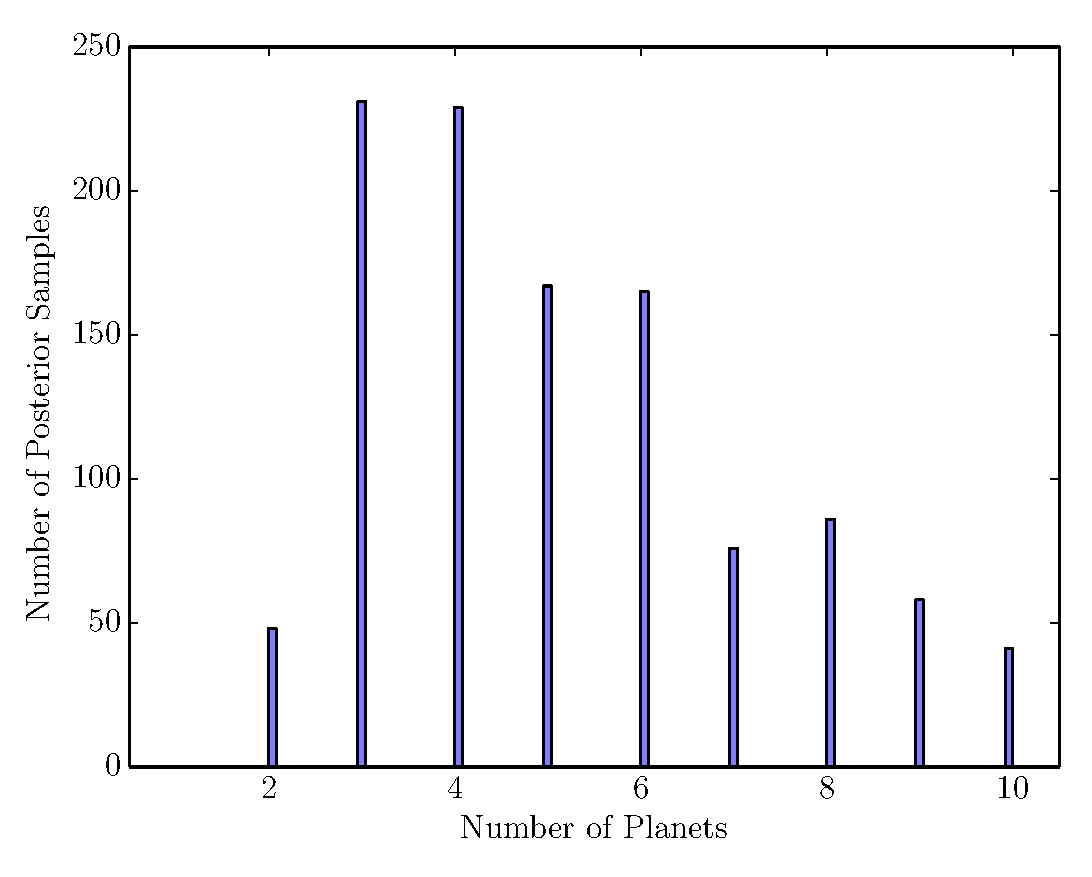
\includegraphics[scale=0.45]{Figures/nu_oph_N.eps}
\caption{The posterior distribution for the number of planets $N$ orbiting
$\nu$ Oph.\label{fig:nu_oph_N}}
\end{figure}

\begin{figure}
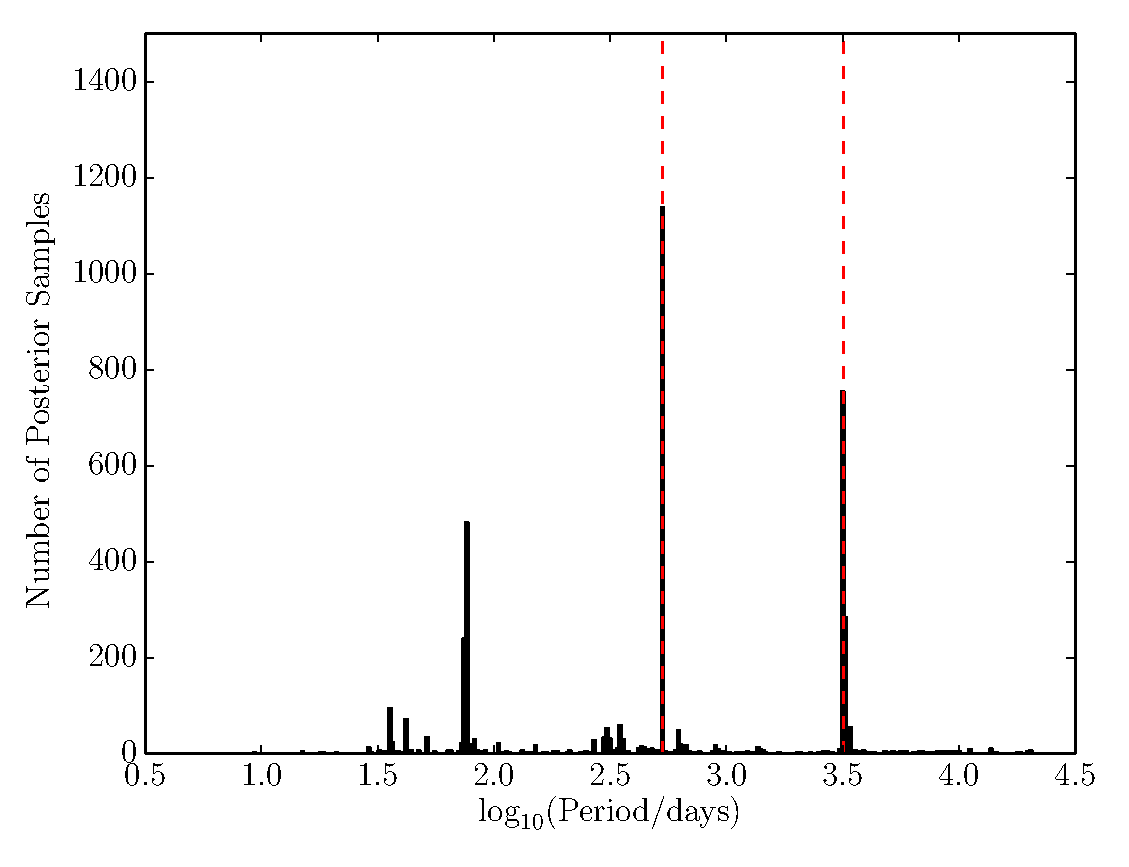
\includegraphics[scale=0.45]{Figures/nu_oph_periods.eps}
\caption{The posterior distribution for the orbital periods in the $\nu$ Oph
system.\label{fig:nu_oph_periods}}
\end{figure}

\begin{figure}
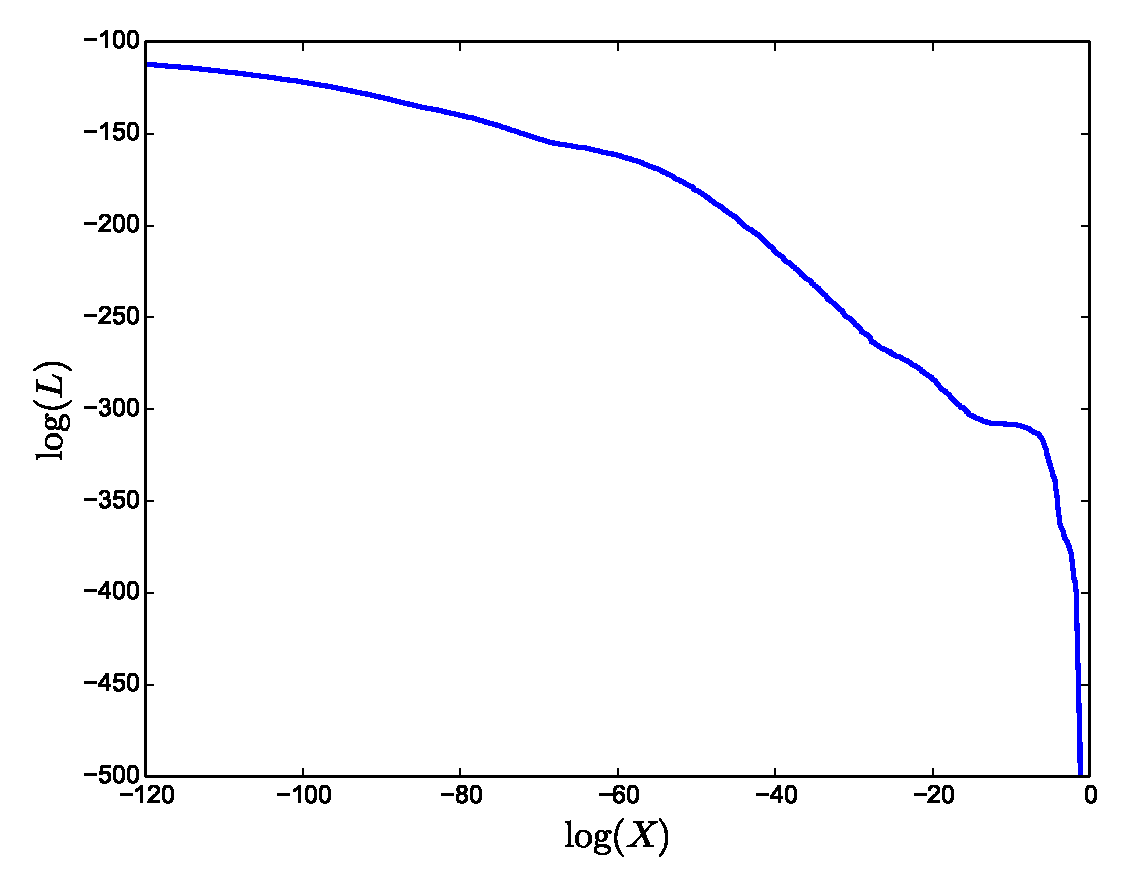
\includegraphics[scale=0.45]{Figures/logl0.eps}
\caption{Log likelihood vs. enclosed prior mass (a standard output of Nested
Sampling algorithms) for the $\nu$ Oph analysis.
There are several phase transitions (concave-up regions) present. The one at
$\log(X) \approx -75$ separates models which contain the third signal from
models that do not. Without using Nested Sampling it would be very difficult
to mix between these two situations and calculate the posterior probability
for the existence of the third signal.
\label{fig:logl0}}
\end{figure}

Figure~\ref{fig:logl0} shows the relationship between the likelihood $L$
and the enclosed prior mass $X$ for the $\nu$ Oph analysis. These plots are
a standard output of Nested Sampling \citep{skilling} analyses, and provide
insights into the structure of the problem. Concave-up regions of this curve
indicate phase transitions which can cause severe problems for annealing-based
methods, and sometimes even for sampling the posterior distribution. In this
analysis, the models with a third signal exist to the left of the phase
transition at $\log(X) \approx -75$, and models without the signal exist to the
right of the phase transition. Mixing between these two phases is crucial for
accurately computing the posterior probability that the third signal exists.
However, if we had simply tried to sample the posterior distribution, it would
not mix between these two phases because the posterior is composed of a
large-volume low-likelihood ``slab'' and a low-volume high-likelihood ``spike''.
It is difficult for standard MCMC methods to escape the spike because of the
likelihood contrast, and it is also difficult to escape the slab and enter the
spike because of its small volume. Thus, even unimodal posterior distributions
can cause mixing problems analogous to multimodal situations if a phase
transition is present.

The marginal likelihood for our model was
$\ln(\mathcal{Z}) \approx -217.04$ and the information
(Kullback-Leibler divergence from the prior to the posterior)
was $\mathcal{H} \approx 80.0$ nats.

\section{Reanalysis of Gliese 581}
The red dwarf star Gliese 581 is thought to host several planets. Exactly
how many is a matter of considerable debate. According to
\citet{2014Sci...345..440R}, there are two planets
(b and c, with periods 5.36 and 12.91 days respectively)
whose existence is generally
accepted, two more
(d and e, with periods 66 and 3.15 days respectively)
whose existence is mostly accepted, and another two
(f and g, with periods 433 and 36.5 days respectively)
whose existence is generally doubted.
To run our code on the combined dataset from the HARPS and HIRES spectrographs,
we extended the model to include separate DC offsets for each instrument, as
well as separate ``extra noise'' parameters $s_0$ and $\nu$.

The posterior distribution for $N$ is shown in Figure~\ref{fig:gliese581_N},
and shows strong evidence for at least eight periods
($P(N \leq 7 | \bdata) = 0.004$).
It is now recognised that
there are many possible sources for oscillations in a data set and not all
such oscillations should be claimed as planets \citep{2014Sci...345..440R}. 
Our model cannot distinguish between oscillations due to planets and
oscillations due to stellar activity: any oscillations found in the dataset
will be described as ``planets'' by the model. However it is interesting that
we find many more signals in the data than previous authors.

By inspecting the posterior distribution for the periods
(Figure~\ref{fig:gliese581_periods}), we see that only four of the periods
are well determined, corresponding to the known periods of Gliese 581 b, c, d,
and e. The other ``periods'' are very uncertain. It is possible that a
non-sinusoidal signal due to stellar activity is being modelled as several
periods \citep{astero}, and if the model were extended to include a ``stochastic''
oscillation \citep{gaussproc}, the number of periods detected may be reduced
substantially.

\begin{figure}
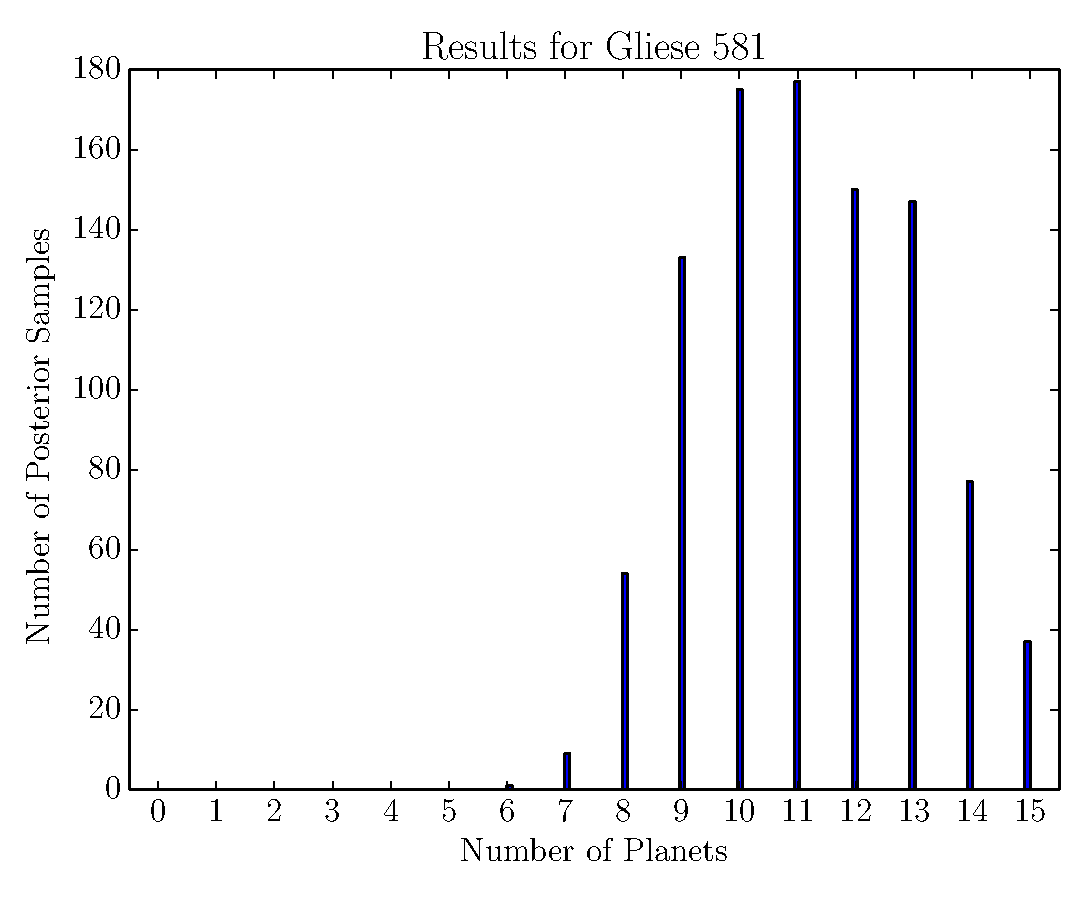
\includegraphics[scale=0.45]{Figures/gliese581_N.eps}
\caption{The posterior distribution for the number of planets $N$ orbiting
Gliese 581.\label{fig:gliese581_N}}
\end{figure}

\begin{figure}
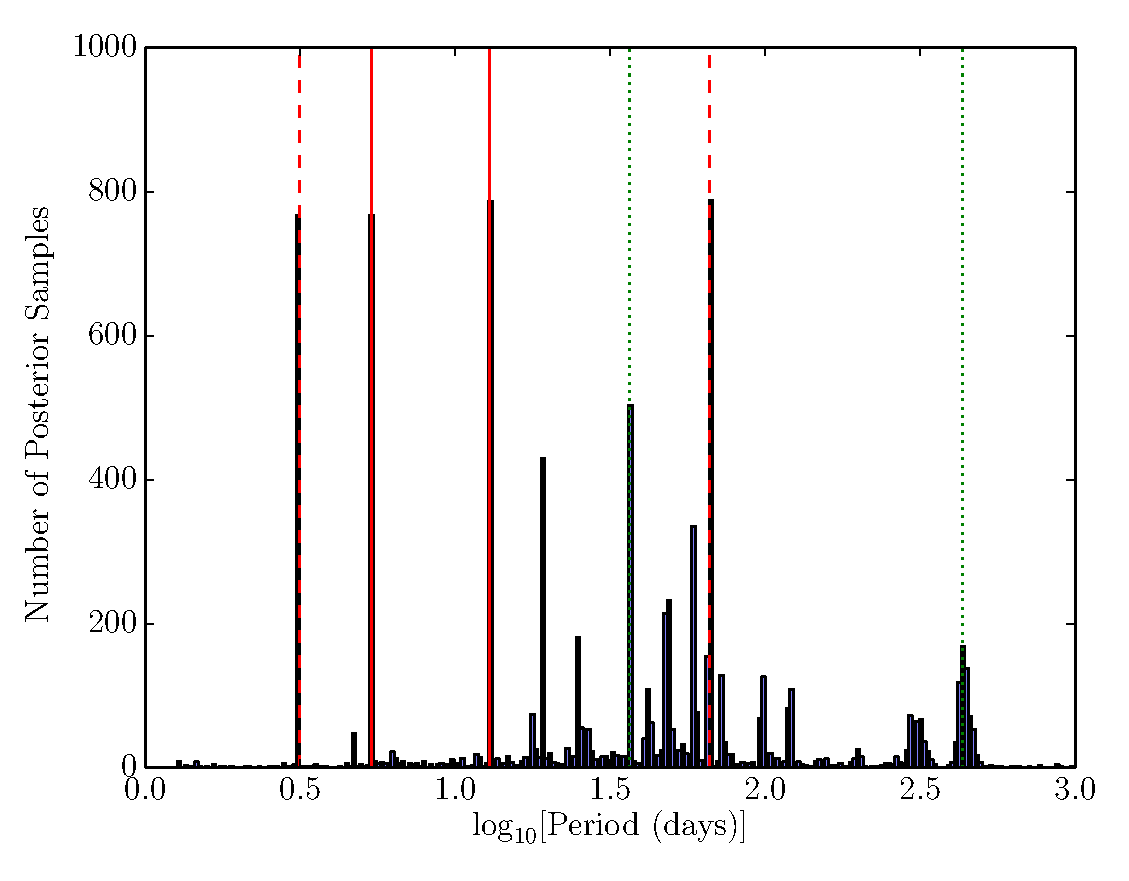
\includegraphics[scale=0.45]{Figures/gliese581_periods.eps}
\caption{The posterior distribution for the orbital periods in the Gliese 581
system.\label{fig:gliese581_periods}}
\end{figure}

The marginal likelihood was $\ln(\mathcal{Z}) \approx -618.04$ and the
information was $\mathcal{H} \approx 140.2$ nats. This compares favourably
to the marginal likelihood of $-640.1$ (for a 6-planet model)
found by \citet{fengji}, although it is unclear whether we used exactly the
same dataset.
Interestingly, the log-likelihood curve (Figure~\ref{fig:logl})
shows this problem has two phase transitions. While these do not affect the
posterior distribution (as they did for $\nu$ Oph), they would cause difficulties
if we tried to calculte the marginal likelihood using thermal annealing.

\begin{figure}
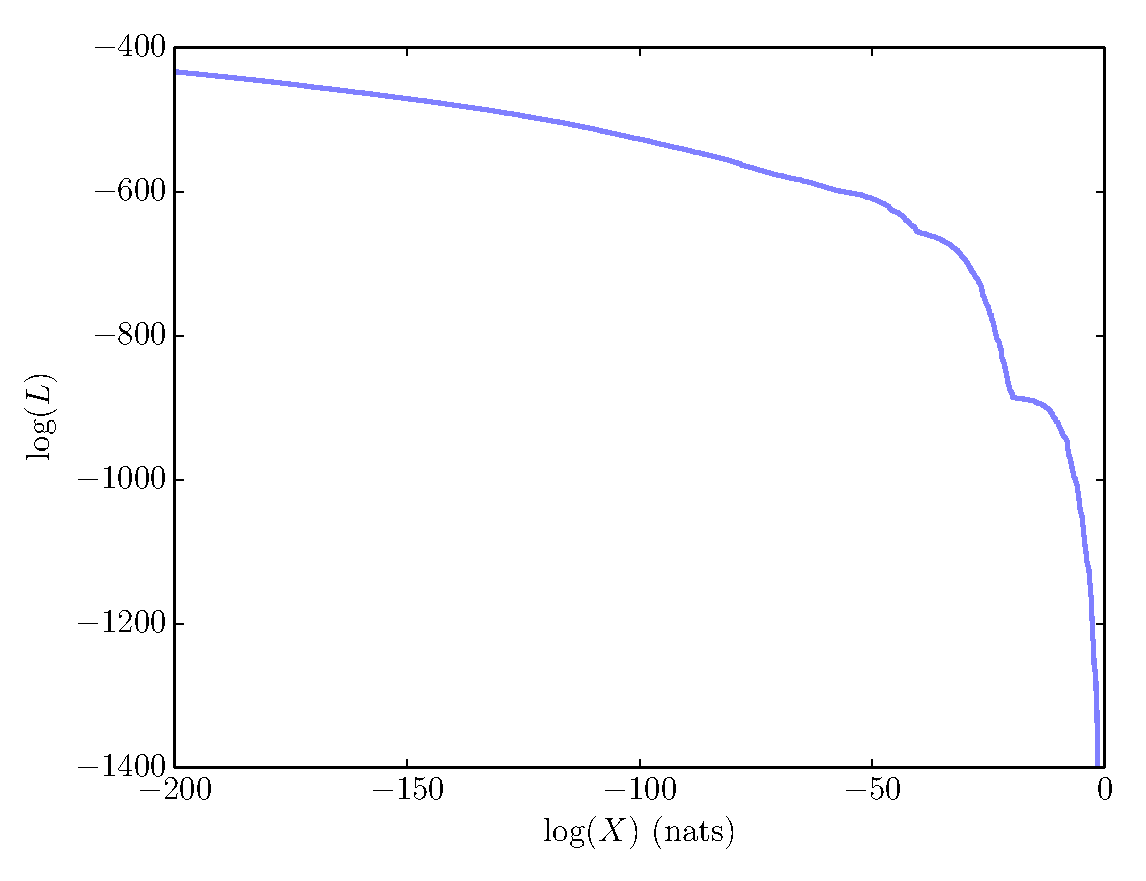
\includegraphics[scale=0.45]{Figures/logl.eps}
\caption{Log likelihood vs. enclosed prior mass for the Gliese 581 analysis.
The two concave-up regions (at $\log(X) \approx -25$ and -45) correspond to
phase transitions. Thermal approaches to this problem would produce misleading
estimates of the marginal likelihood because they would mix poorly at temperatures
around 11 and 4.
\label{fig:logl}}
\end{figure}


\section{Conclusions}
In this paper we introduced a trans-dimensional MCMC approach to inferring
the number of planets $N$ in an exoplanetary system from radial velocity data.
The MCMC was implemented using the framework of \citet{rjobject} which
defines trans-dimensional birth and death moves, and does the sampling
with respect to a Nested Sampling target distribution, rather than directly
sampling the posterior. This approach allows us to compute the results in a
single run, which provides posterior samples and an estimate of the marginal
likelihood. By embedding the MCMC in a Nested Sampling algorithm, instead of
directly trying to sample the posterior distribution, we can overcome difficult
features in the problem, such as phase transitions.

We applied the code to two well-studied RV datasets, $\nu$ Oph and Gliese 581.
In $\nu$ Oph, we found some evidence for a signal with a period of
75.7 $\pm$ 1.8 days: the posterior probability it exists, given our assumptions,
is 70\%. The posterior distribution contains models with three signals and
models with two, however, these are separated by a phase transition. Therefore
mixing between the two situations would be very difficult if we simply tried
to sample the posterior distribution.

With the combined HIRES+HARPS dataset from Gliese 581, we found
evidence for a large number of ``planets'', although only four have well
determined periods, corresponding to the Gliese 581 b, c, d,
and e. Since our model does not include any possibility of stellar variability,
any such periodic signals will be attributed to ``planets''.
Including non-planetary stellar variability is a crucial next step.

\vspace{-0.5cm}
\section*{Acknowledgements}
It is a pleasure to thank Fengji Hou and David Hogg (NYU) for inspiring me to
finally work on this problem, and Phil Gregory (UBC) for writing so many
interesting papers on it. Tom Loredo (Cornell) also provided interesting
conversations. This work was supported by a Marsden Fast Start
grant from the Royal Society of
New Zealand.

\begin{thebibliography}{99}
\bibitem[\protect\citeauthoryear{Batalha}{2014}]{2014PNAS..11112647B} 
Batalha N.~M., 2014, PNAS, 111, 12647 

\bibitem[\protect\citeauthoryear{Bennett et 
al.}{2014}]{2014ApJ...785..155B} Bennett D.~P., et al., 2014, ApJ, 785, 155 

\bibitem[\protect\citeauthoryear{Brewer 
\& Stello}{2009}]{gaussproc} Brewer B.~J., Stello D., 2009, MNRAS, 395, 2226 

\bibitem[\protect\citeauthoryear{Brewer et al.}{2007}]{astero} 
Brewer B.~J., Bedding T.~R., Kjeldsen H., Stello D., 2007, ApJ, 654, 551 

\bibitem[\protect\citeauthoryear{Brewer, P{\'a}rtay,
\& Cs{\'a}nyi}{2011}]{dnest} Brewer B.~J., P{\'a}rtay L.~B., Cs{\'a}nyi G., 2011,
Statistics and Computing, 21, 4, 649-656. arXiv:0912.2380

\bibitem[\protect\citeauthoryear{Brewer}{2014}]{rjobject} Brewer, B. J., 2014,
Bayesian Analysis, submitted.

\bibitem[\protect\citeauthoryear{Feroz 
\& Hobson}{2014}]{2014MNRAS.437.3540F} Feroz F., Hobson M.~P., 2014, MNRAS, 437, 3540 

\bibitem[\protect\citeauthoryear{Feroz, Balan, 
\& Hobson}{2011}]{2011MNRAS.415.3462F} Feroz F., Balan S.~T., Hobson M.~P., 2011, MNRAS, 415, 3462

\bibitem[\protect\citeauthoryear{Green}{1995}]{green}
Green, P.~J., 1995, Reversible Jump Markov Chain Monte Carlo Computation and Bayesian Model Determination, Biometrika 82 (4): 711–732.

\bibitem[\protect\citeauthoryear{Gregory}{2011}]{2011MNRAS.415.2523G} 
Gregory P.~C., 2011, MNRAS, 415, 2523 

\bibitem[\protect\citeauthoryear{Gregory}{2011}]{2011MNRAS.410...94G} 
Gregory P.~C., 2011, MNRAS, 410, 94 

\bibitem[\protect\citeauthoryear{Hou, Goodman, 
\& Hogg}{2014}]{fengji} Hou F., Goodman J., Hogg D.~W., 2014, arXiv, arXiv:1401.6128 

\bibitem[\protect\citeauthoryear{Neal}{2001}]{neal}
Neal, R.~M., 2001, Statistics and Computing 11.2, 125-139.

\bibitem[\protect\citeauthoryear{O'Hagan and Forster}{2004}]{ohagan}
O'Hagan, A., Forster,~J., 2004, Bayesian inference. London: Arnold.

\bibitem[\protect\citeauthoryear{Quirrenbach, Reffert, 
\& Bergmann}{2011}]{2011AIPC.1331..102Q} Quirrenbach A., Reffert S., Bergmann C., 2011, AIPC, 1331, 102 

\bibitem[\protect\citeauthoryear{Robertson et 
al.}{2014}]{2014Sci...345..440R} Robertson P., Mahadevan S., Endl M., Roy 
A., 2014, Sci, 345, 440 

\bibitem[\protect\citeauthoryear{Sato et al.}{2012}]{2012PASJ...64..135S} 
Sato B., et al., 2012, PASJ, 64, 135 

\bibitem[\protect\citeauthoryear{Sivia \& Skilling}{2006}]{sivia} Sivia, 
D.~ S., Skilling, J., 2006, Data Analysis: A Bayesian Tutorial, 2nd 
Edition, Oxford University Press

\bibitem[\protect\citeauthoryear{Skilling}{2006}]{skilling} Skilling, 
J., 2006, ``Nested Sampling for General Bayesian Computation'', Bayesian 
Analysis 4, pp. 833-860

\bibitem[Stephens(2000)]{birthdeath} Stephens, M., 2000, ``Bayesian analysis of mixture models with an unknown number of components-an alternative to reversible jump methods.'', Annals of Statistics, 40-74.

\bibitem[\protect\citeauthoryear{Tuomi}{2011}]{2011A&A...528L...5T} Tuomi M., 2011, A\&A, 528, L5 

\bibitem[\protect\citeauthoryear{Umst{\"a}tter et 
al.}{2005}]{umstatter} Umst{\"a}tter R., Christensen N., Hendry 
M., Meyer R., Simha V., Veitch J., Vigeland S., Woan G., 2005, PhRvD, 72, 
022001 

\bibitem[\protect\citeauthoryear{Yee et al.}{2014}]{2014ApJ...790...14Y} 
Yee J.~C., et al., 2014, ApJ, 790, 14 

\bibitem[\protect\citeauthoryear{Zechmeister \& K{\"u}rster}{2009}]{2009A&A...496..577Z} Zechmeister M., K{\"u}rster M., 2009, A\&A, 496, 577  

\end{thebibliography}



\end{document}

%%%%%%%%%%%%%%%%%%%%%%%%%%%%%%%%%%%%%%%%%%%%%%%%%%%%%%%%%%%%%%%%%%%%%%%%%%%%%%
